\documentclass[final]{article}
\usepackage[paperwidth=33.1in,paperheight=23.4in,margin=0.6in]{geometry}
\usepackage{graphicx}
\usepackage{multicol}
\usepackage{booktabs}
\usepackage{xcolor}
\usepackage{tikz}
\usepackage{amsmath}
\usepackage{enumitem}
\usepackage{helvet}
\renewcommand{\familydefault}{\sfdefault}

% Colors matching template
\definecolor{headerblue}{HTML}{4FC1C9}
\definecolor{footerblue}{HTML}{4FC1C9}
\definecolor{sectiongray}{HTML}{C0C0C0}
\definecolor{darktext}{HTML}{222222}
\definecolor{boxborder}{HTML}{88CCCC}

\pagestyle{empty}
\setlength{\parindent}{0pt}
\setlength{\parskip}{0.4em}
\setlist[itemize]{leftmargin=1.2em,itemsep=0.2em,parsep=0em,topsep=0.2em}

% Section heading command
\newcommand{\postersection}[1]{%
  \vspace{0.3em}%
  {\colorbox{sectiongray}{\makebox[\linewidth][l]{\textbf{\large\color{darktext} #1}}}}%
  \vspace{0.3em}%
}

\begin{document}

% ============================================================================
% HEADER BAR
% ============================================================================
\noindent
\begin{tikzpicture}[remember picture, overlay]
  \fill[headerblue] (current page.north west) rectangle ([yshift=-2.8in]current page.north east);
  % Title text — positioned lower so it's clearly within the bar
  \node[anchor=north west, text width=25in, font=\bfseries\fontsize{48}{56}\selectfont, text=white] 
    at ([xshift=0.6in, yshift=-0.5in]current page.north west) 
    {Movie Memory Test: Effects of Boundary Type on Recognition, Signal Detection, and Metacognition};
  % BRSM badge — white background box in top right corner
  \node[anchor=north east, text width=5in, font=\bfseries\fontsize{24}{30}\selectfont, text=darktext, align=center, fill=white, inner sep=12pt] 
    at ([xshift=-0.6in, yshift=-0.3in]current page.north east) 
    {BRSM PROJECT\\POSTER\\PRESENTATION SP\\2026};
\end{tikzpicture}

% ============================================================================
% FOOTER BAR
% ============================================================================
\begin{tikzpicture}[remember picture, overlay]
  \fill[footerblue] (current page.south west) rectangle ([yshift=0.7in]current page.south east);
  \node[anchor=south west, font=\bfseries\itshape\fontsize{22}{26}\selectfont, text=darktext] 
    at ([xshift=0.7in, yshift=0.15in]current page.south west) 
    {Archit Choudhary (2023114002), Bhavya Ahuja (2023111035), Hrishiraj Mitra (2023111037)};
  \node[anchor=south east, font=\bfseries\itshape\fontsize{22}{26}\selectfont, text=darktext] 
    at ([xshift=-0.7in, yshift=0.15in]current page.south east) 
    {Team Odomos | IIIT Hyderabad};
\end{tikzpicture}

\vspace*{2.9in}

% ============================================================================
% MAIN CONTENT — 3 columns matching template
% ============================================================================
\fontsize{18}{22}\selectfont

\begin{minipage}[t]{0.22\textwidth}

% ====== LEFT COLUMN: ABSTRACT + METHODOLOGY ======

\postersection{ABSTRACT}

This study investigates how boundary type (Abrupt Cut vs.\ Natural Cut) and target frame type (Event-Model vs.\ Boundary-Break) affect recognition memory for movie clips. 170 participants viewed 40 clips and completed a 2AFC recognition task. We found that natural event segmentation preserves memory encoding ($d = 0.41$), while the predicted boundary advantage (BB $>$ EM) was not observed. Signal Detection Theory confirmed the NB advantage reflects genuine discriminability ($d' = 2.26$ vs.\ $2.01$). Abrupt boundaries selectively impair metacognitive certainty for boundary-adjacent content while accuracy remains comparable.

\vspace{0.3em}

\postersection{METHODOLOGY}

\textbf{Design:} 2 (Boundary Type: AB vs.\ NB; between) $\times$ 2 (Target Type: EM vs.\ BB; within) mixed design.

\textbf{Analytical Pipeline:}
\begin{itemize}
  \item Descriptive statistics and assumption checks (Shapiro-Wilk, Levene's)
  \item 2$\times$2 Mixed ANOVA with $\eta_p^2$
  \item Non-parametric robustness checks (Mann-Whitney, Wilcoxon)
  \item Signal Detection Theory: $d'$ and criterion $c$ with log-linear correction
  \item Mixed-effects models with crossed random effects (subjects $\times$ items)
  \item Demographic moderation (ANCOVA)
  \item Bayesian analysis for near-significant effects
\end{itemize}

\textbf{Missing Data:} Demographics for 22 participants imputed using \textbf{median} (age) and \textbf{mode} (categoricals).

\vspace{0.5em}

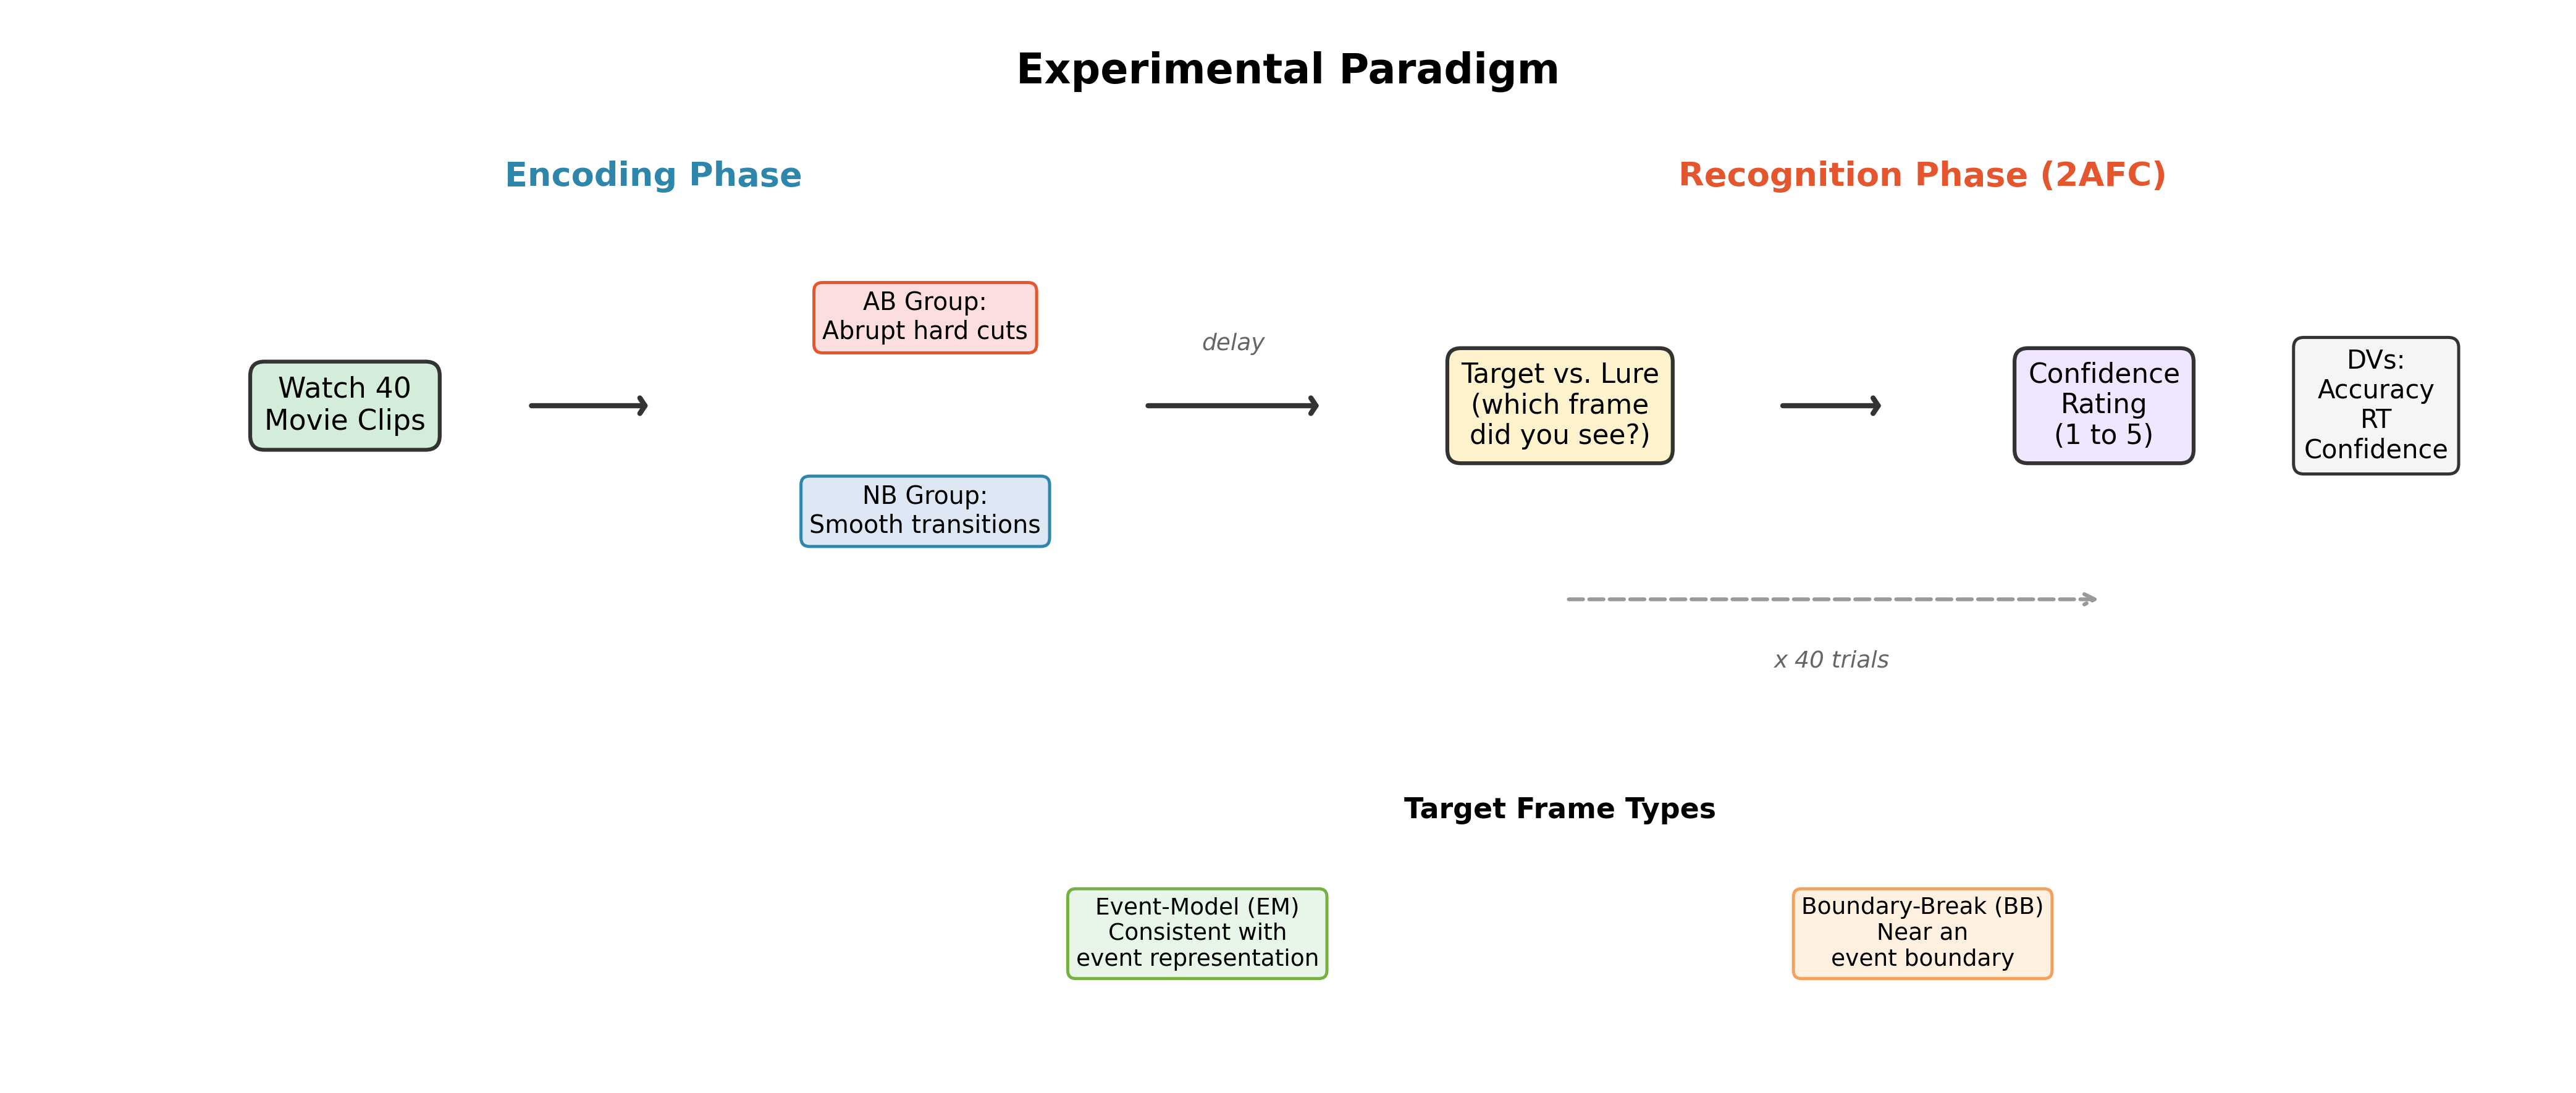
\includegraphics[width=\linewidth]{output/fig8_task_paradigm.png}

{\small\textit{Figure 1: Experimental paradigm — encoding $\rightarrow$ 2AFC recognition $\rightarrow$ confidence.}}

\end{minipage}%
\hfill%
\begin{minipage}[t]{0.50\textwidth}

% ====== CENTER COLUMN: RESULTS ======

\postersection{RESULTS}

\textbf{H1 (NB $>$ AB Accuracy): Supported.} Mixed ANOVA: $F(1,168) = 7.25$, $p = .008$, $\eta_p^2 = .041$. NB ($M = .871$) outperformed AB ($M = .840$), Cohen's $d = 0.41$ (medium effect). Non-parametric Mann-Whitney confirmed: $U = 2744$, $p = .007$.

\textbf{H2 (BB $>$ EM Boundary Advantage): Not Supported.} $F(1,168) = 11.44$, $p < .001$, $\eta_p^2 = .064$. \textbf{Direction reversed}: EM ($M = .870$) $>$ BB ($M = .843$). The boundary advantage (Radvansky \& Zacks, 2017) does not hold when boundaries are artificially disrupted.

\vspace{0.3em}

\begin{minipage}[t]{0.48\linewidth}
  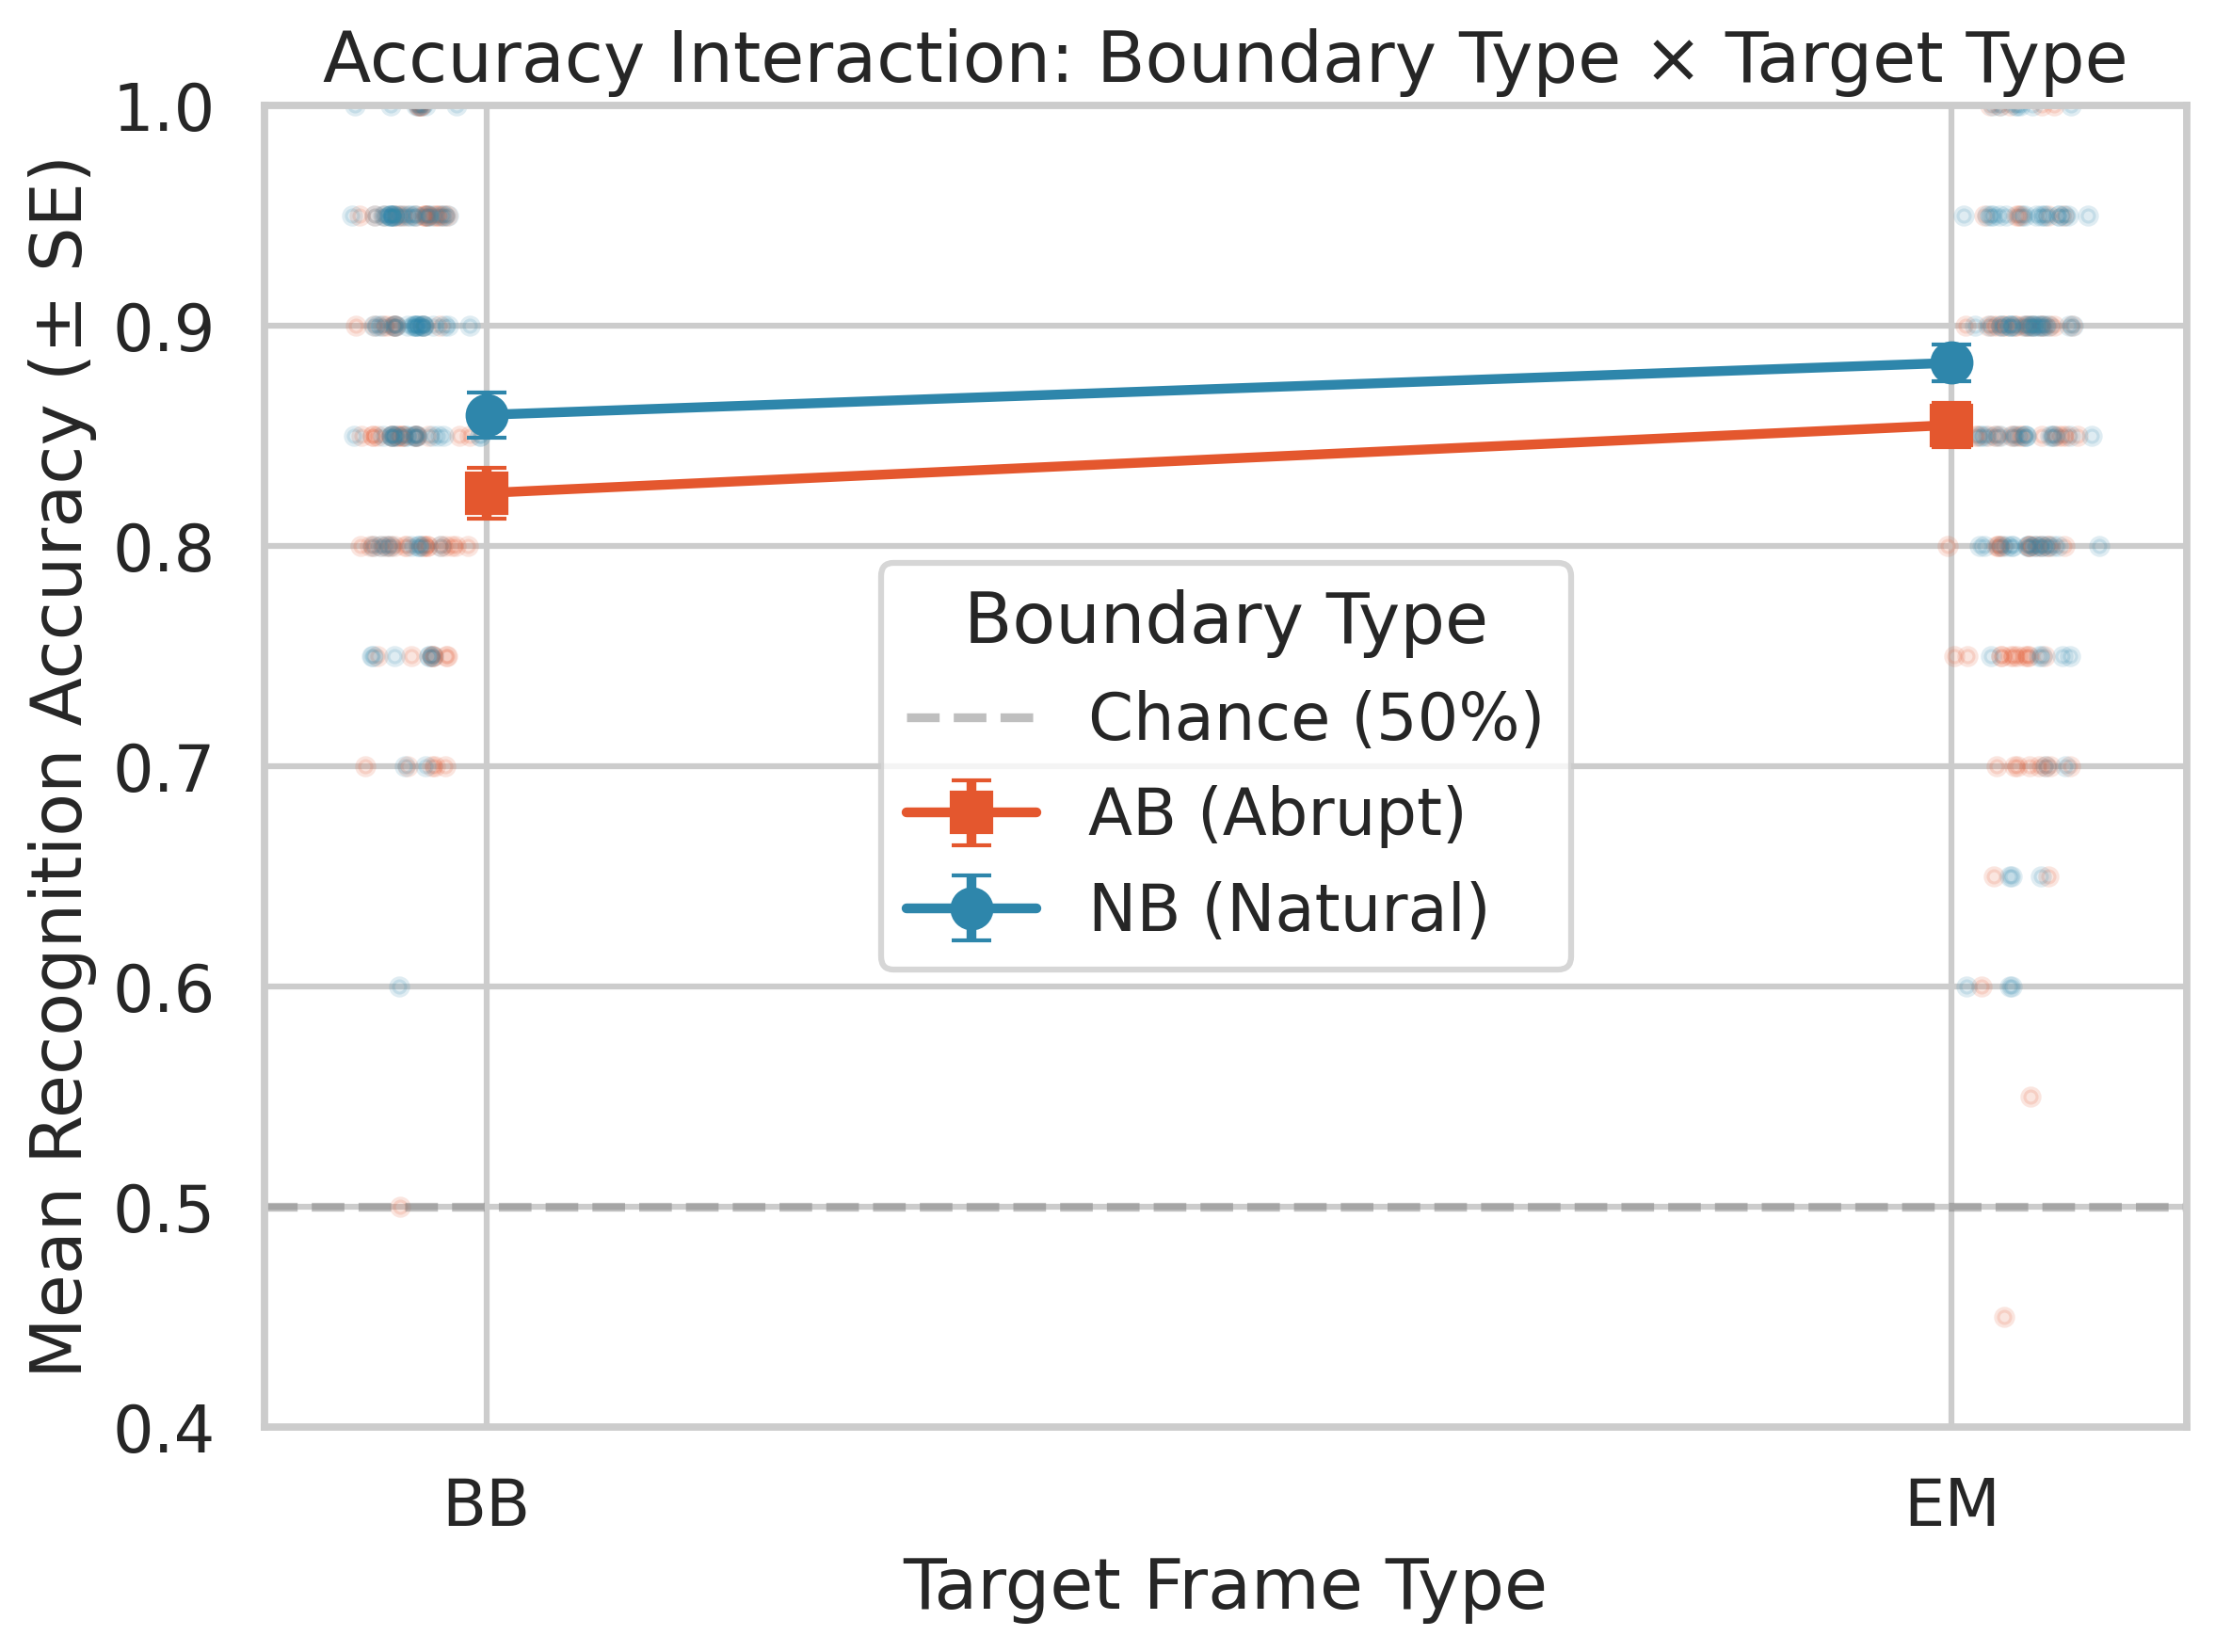
\includegraphics[width=\linewidth]{output/fig1_accuracy_interaction.png}
  {\small\textit{Figure 2: Accuracy interaction with individual data.}}
\end{minipage}%
\hfill%
\begin{minipage}[t]{0.48\linewidth}
  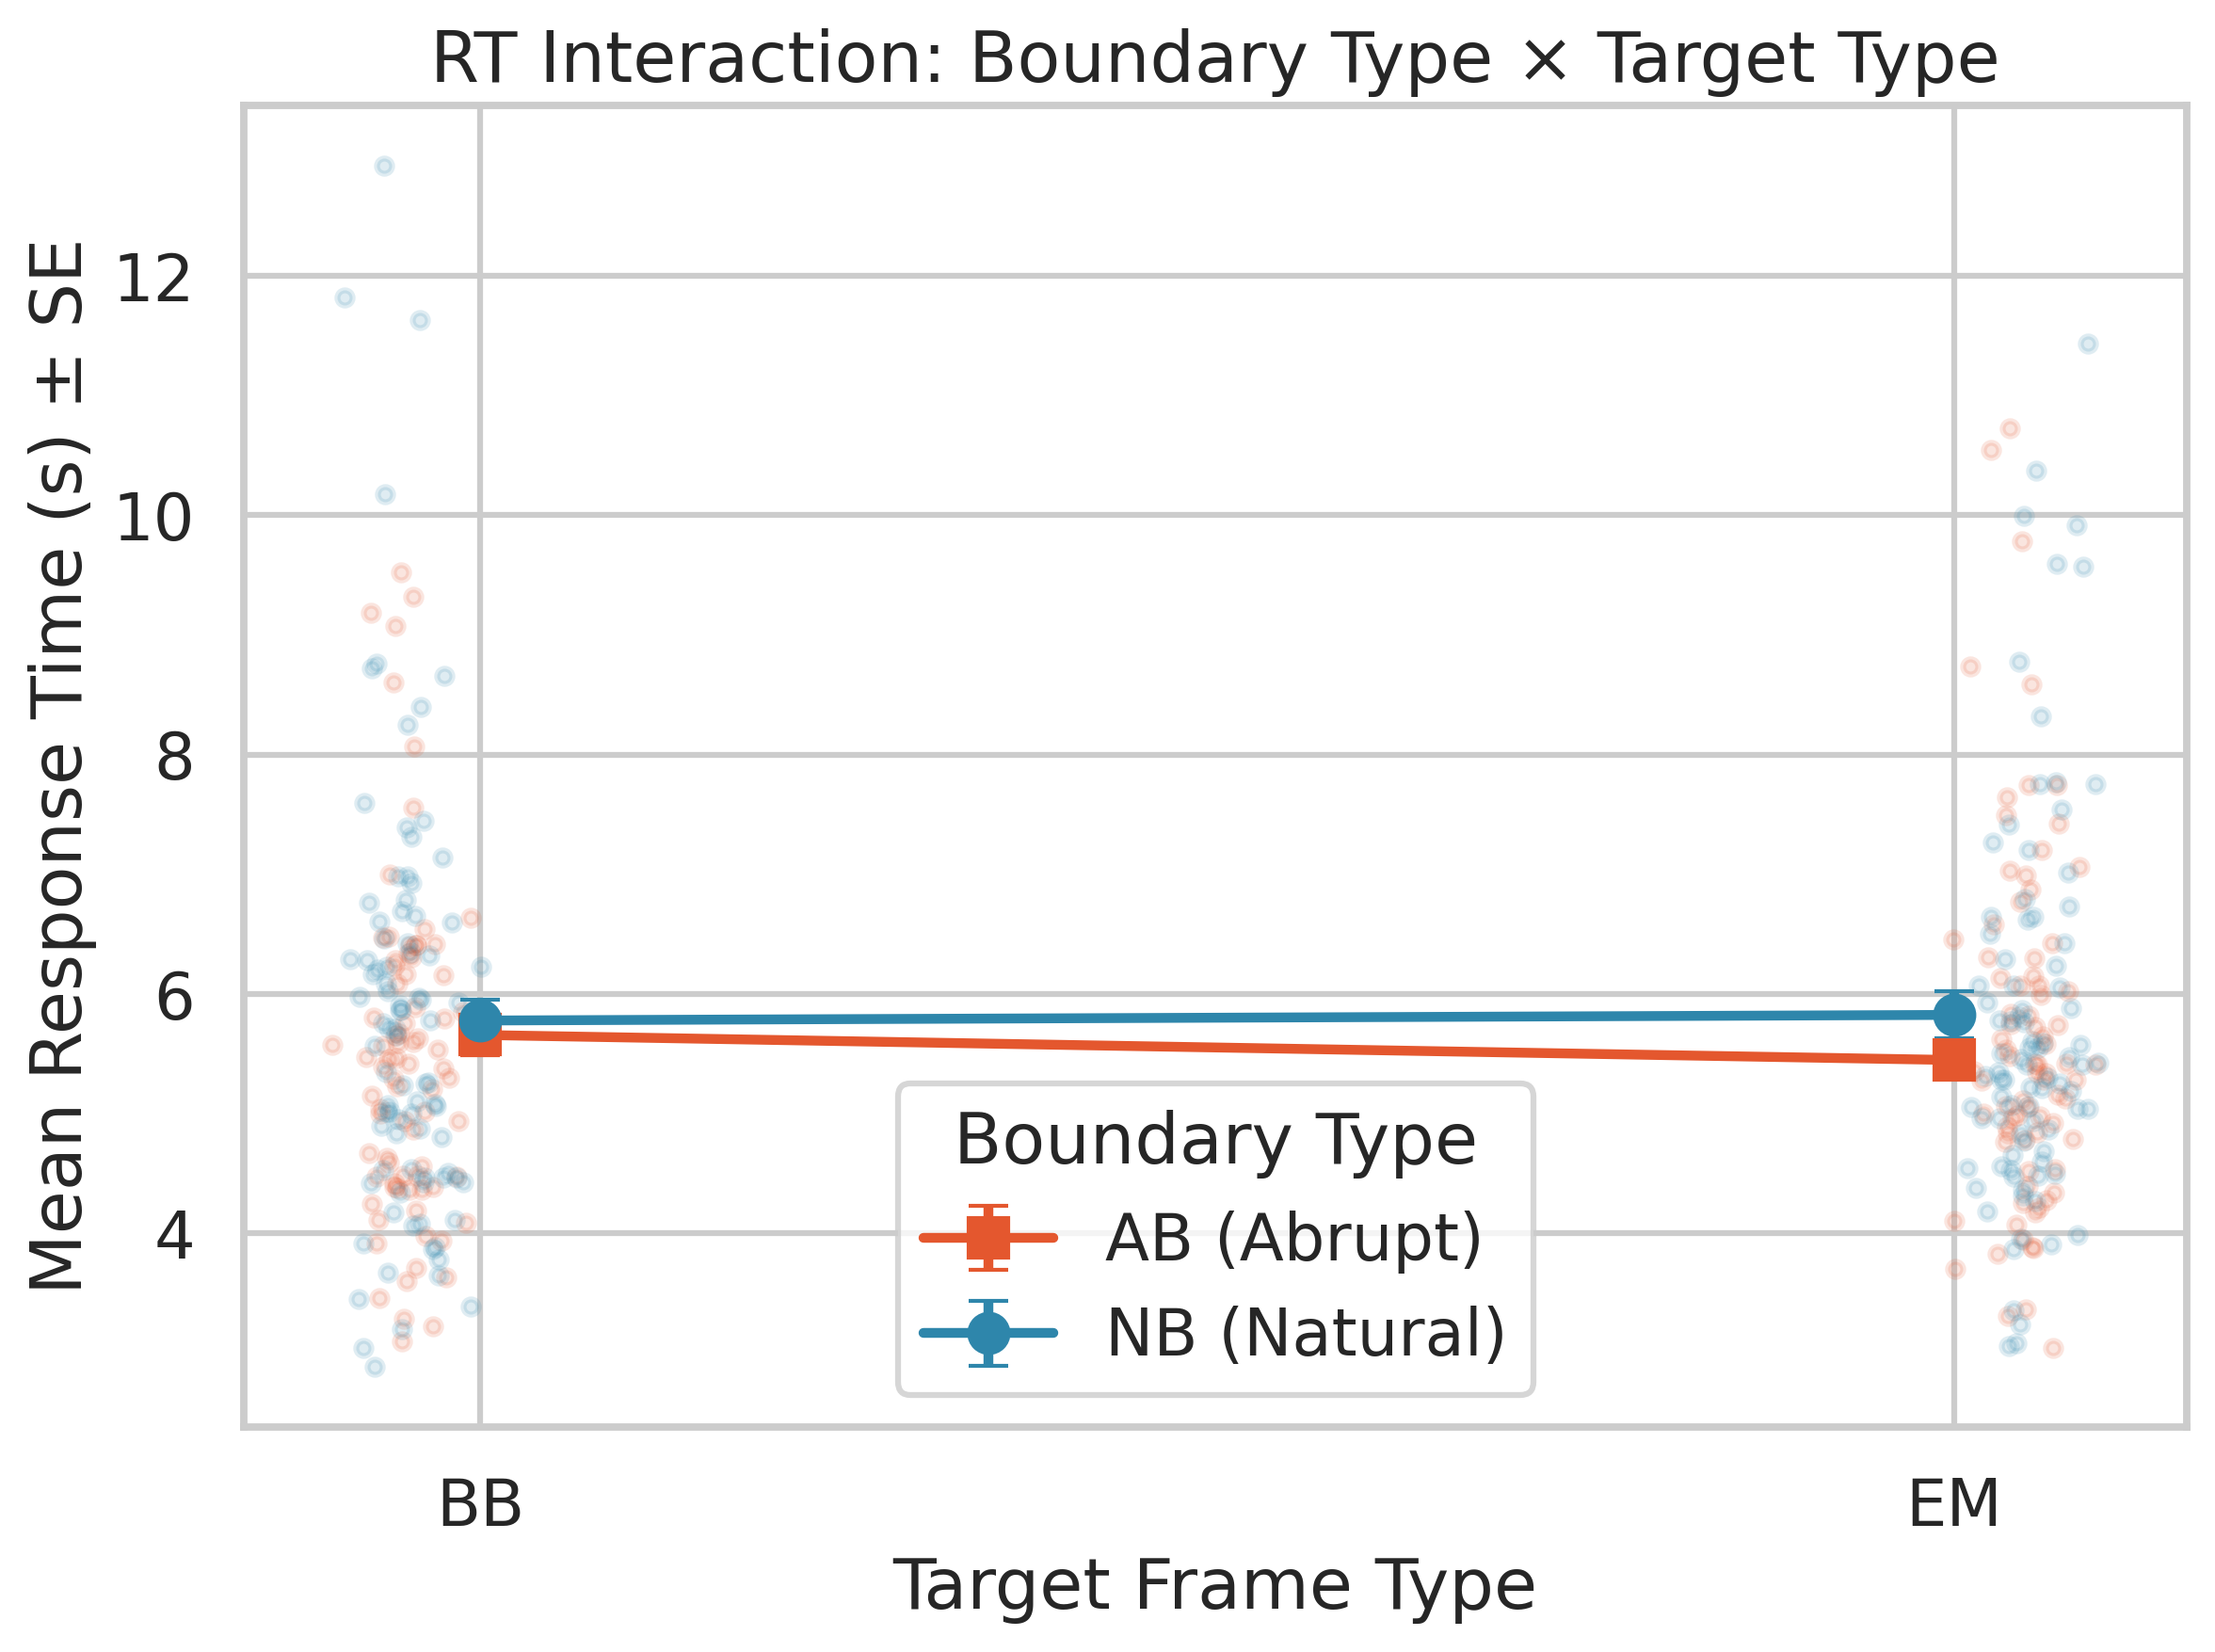
\includegraphics[width=\linewidth]{output/fig10_rt_interaction.png}
  {\small\textit{Figure 3: RT interaction with individual data.}}
\end{minipage}

\vspace{0.4em}

\textbf{H4 (RT Interaction): Partially Supported.}
Omnibus: $F(1,168) = 3.36$, $p = .069$. Simple effects: AB group was significantly slower for BB than EM ($t = -2.56$, $p = .012$, $d = -0.15$); NB showed no difference ($p = .67$). Bayesian BF$_{10} = 0.78$ (anecdotal evidence).

\textbf{H5 (SDT $d'$): Supported.} NB $d' = 2.26$ vs.\ AB $d' = 2.01$; $t = 2.55$, $p = .012$, $d = 0.39$. The NB advantage reflects genuine discriminability (criterion $c$ is undefined in 2AFC).

\vspace{0.3em}

\begin{minipage}[t]{0.48\linewidth}
  \textbf{\large Confidence Interaction}

  Significant interaction $F(1,168) = 4.03$, $p = .046$.
  \begin{itemize}
    \item AB: EM $>$ BB ($p = .003$, $d = .19$)
    \item NB: EM $\approx$ BB ($p = .733$)
    \item BB: NB $>$ AB ($p = .024$, $d = .35$)
  \end{itemize}
  Abrupt cuts impair \textbf{metacognitive certainty} for boundary-adjacent content.
\end{minipage}%
\hfill%
\begin{minipage}[t]{0.48\linewidth}
  \textbf{\large Mixed-Effects Models}

  Crossed random effects (subjects $\times$ items):
  \begin{itemize}
    \item Condition: $b = .036$, $z = 2.95$, $p = .003$
    \item Target Type: $b = .031$, $z = 2.51$, $p = .012$
    \item Interaction: $b = -.007$, $p = .669$
  \end{itemize}
  All effects robust to item-level variability.
\end{minipage}

\vspace{0.4em}

\begin{minipage}[t]{0.48\linewidth}
  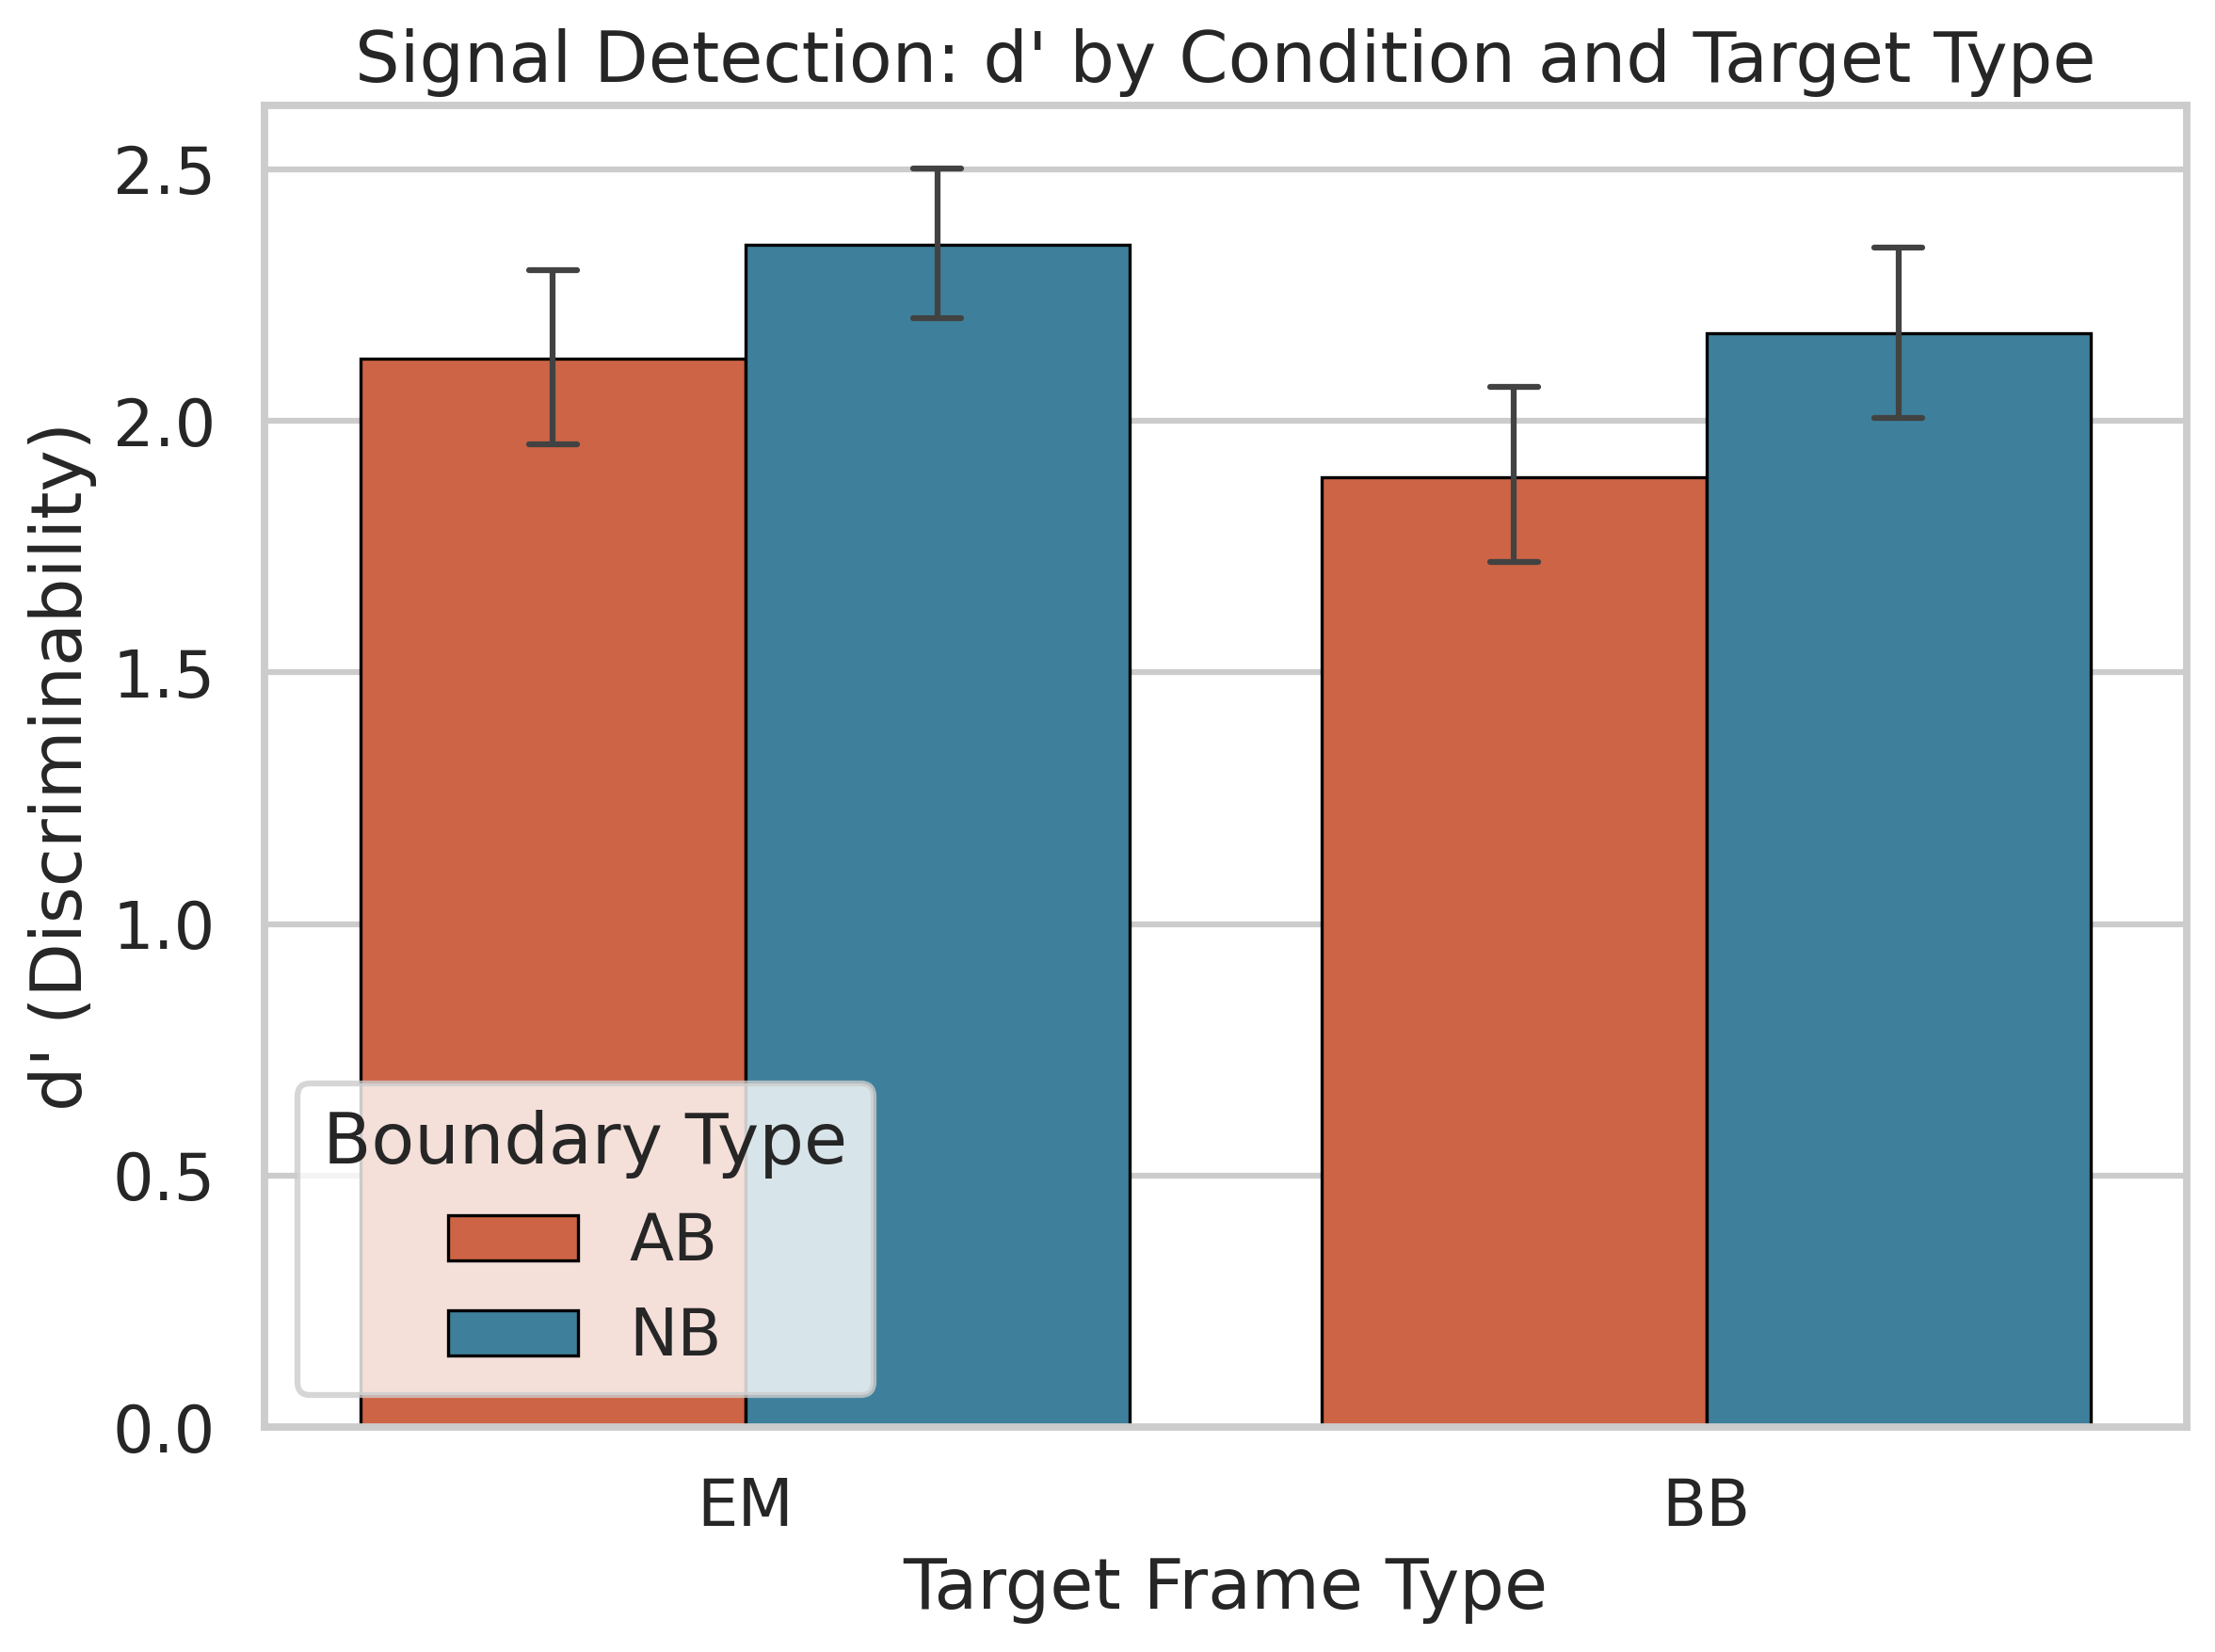
\includegraphics[width=\linewidth]{output/fig9_sdt_dprime.png}
  {\small\textit{Figure 4: SDT $d'$ (discriminability) by condition.}}
\end{minipage}%
\hfill%
\begin{minipage}[t]{0.48\linewidth}
  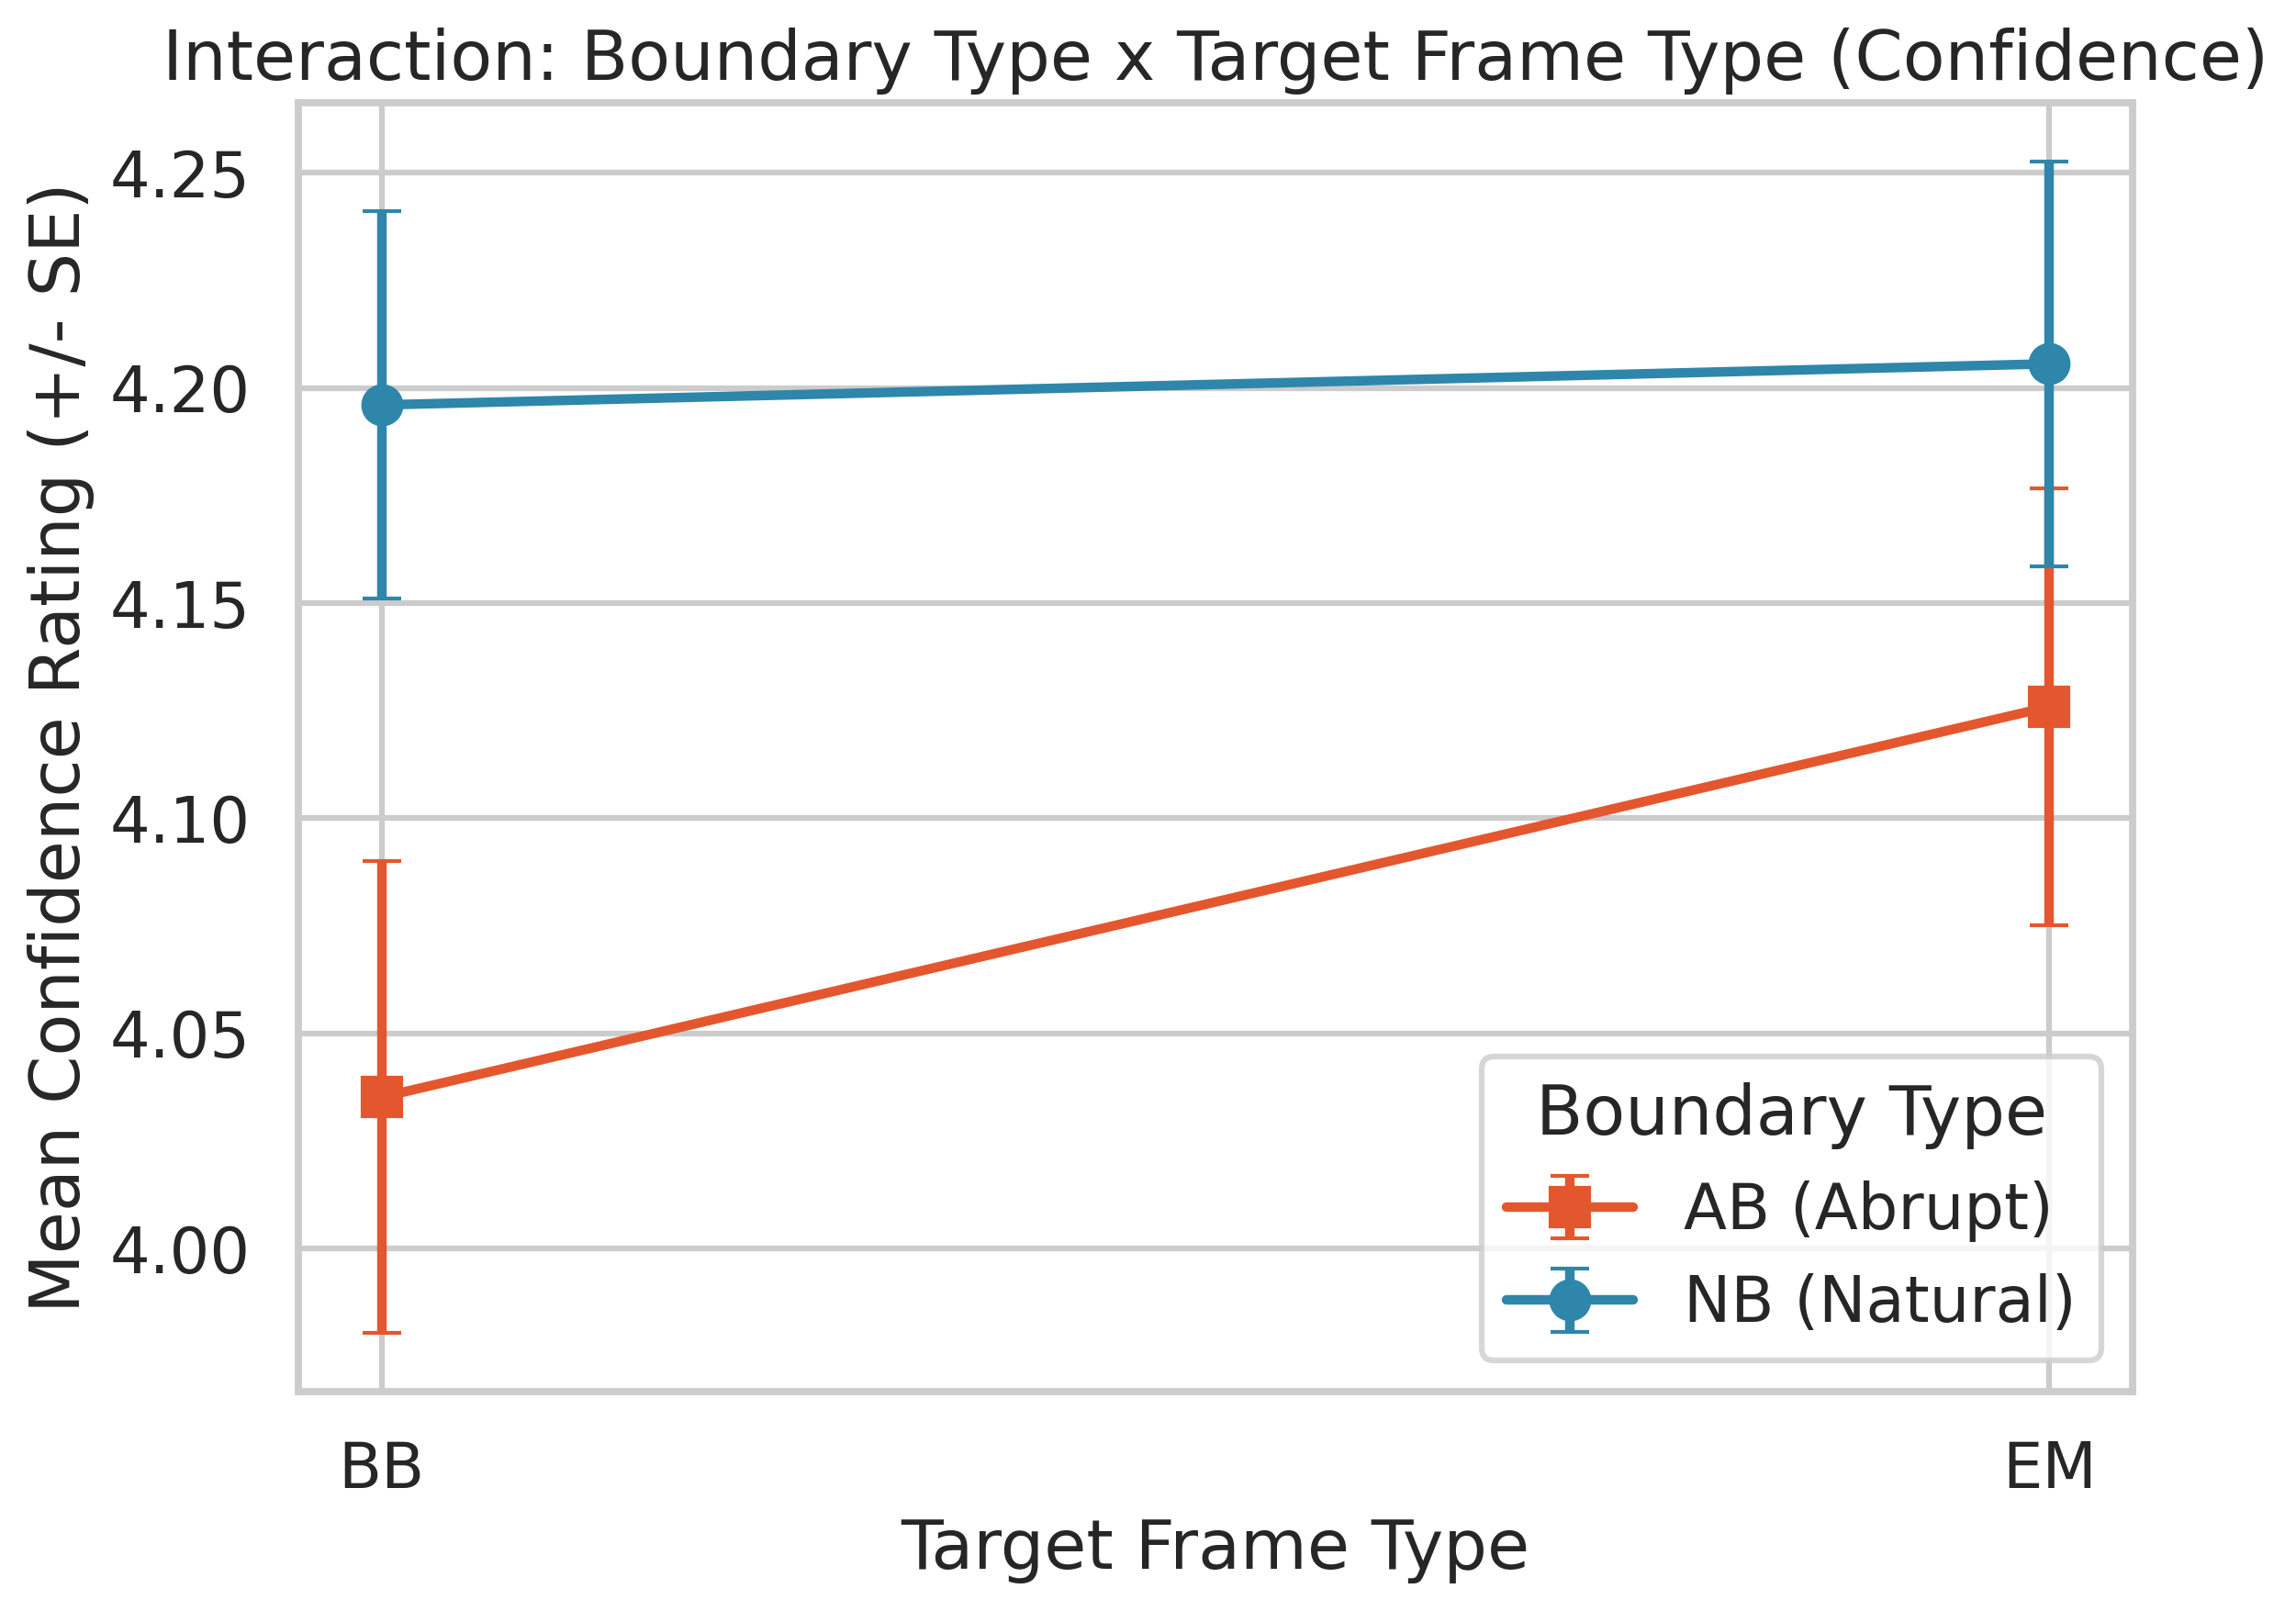
\includegraphics[width=\linewidth]{output/fig7_confidence_interaction.png}
  {\small\textit{Figure 5: Confidence interaction plot.}}
\end{minipage}

\end{minipage}%
\hfill%
\begin{minipage}[t]{0.23\textwidth}

% ====== RIGHT COLUMN: CONCLUSION + ACKNOWLEDGMENT + REFERENCES ======

\postersection{CONCLUSION \& FUTURE WORK}

\textbf{Key findings:}
\begin{enumerate}[leftmargin=1.2em,itemsep=0.15em]
  \item \textbf{Natural boundaries preserve memory}: NB group showed higher accuracy ($d = 0.41$) and discriminability ($d' = 0.39$), supporting Event Segmentation Theory.
  \item \textbf{Boundary advantage fails} when boundaries are artificially disrupted (H2 rejected).
  \item \textbf{Metacognitive dissociation}: AB group was less confident about BB targets while maintaining comparable accuracy — abrupt cuts impair subjective certainty.
  \item \textbf{RT interaction}: AB participants selectively slow down for BB targets, consistent with disrupted event model updating.
  \item \textbf{Demographics}: Age negatively correlated with accuracy ($\rho = -.203$, $p = .008$); effect survives ANCOVA.
\end{enumerate}

\textbf{Future directions:}
\begin{itemize}
  \item Yes/no recognition for richer SDT
  \item Model item-level predictors
  \item Replicate RT interaction
  \item Within-subjects boundary design
\end{itemize}

\vspace{0.4em}

\postersection{HYPOTHESIS SUMMARY}

\fontsize{16}{20}\selectfont

\begin{tabular}{@{}lll@{}}
\toprule
\textbf{H\#} & \textbf{Prediction} & \textbf{Result} \\
\midrule
H1 & NB $>$ AB acc. & \textbf{Supported} \\
H2 & BB $>$ EM & \textbf{Rejected} \\
H3 & Acc. interact. & Not sig. \\
H4 & RT interact. & \textbf{Partial} \\
H5 & NB $d' >$ AB & \textbf{Supported} \\
H6 & Demographics & \textbf{Partial} \\
\bottomrule
\end{tabular}

\fontsize{18}{22}\selectfont

\vspace{0.5em}

\postersection{ACKNOWLEDGMENT}

We thank Dr.\ Gargi Shukla for providing the dataset and experimental design, and the BRSM course instructors for their guidance on statistical methodology.

\vspace{0.5em}

\postersection{REFERENCES}

\fontsize{14}{17}\selectfont

Boltz, M.\ (1992). Temporal accent structure. \textit{JEPHPP}, 18(1), 90--105.

Radvansky, G.\ A., \& Zacks, J.\ M.\ (2017). Event boundaries in memory. \textit{COBS}, 17, 133--140.

Swallow, K.\ M., et al.\ (2009). Event boundaries affect memory encoding. \textit{JEP:G}, 138(2), 236--257.

Zacks, J.\ M., et al.\ (2007). Event perception. \textit{Psych.\ Bull.}, 133(2), 273--293.

Hautus, M.\ J.\ (1995). Corrections for extreme proportions. \textit{BRMIC}, 27(1), 46--51.

\end{minipage}

\end{document}
